\documentclass[10pt,twocolumn]{article} 

% required packages for Oxy Comps style
\usepackage{oxycomps} % the main oxycomps style file
\usepackage{times} % use Times as the default font
\usepackage[style=numeric,sorting=nyt]{biblatex} % format the bibliography nicely

\usepackage{amsfonts} % provides many math symbols/fonts
\usepackage{listings} % provides the lstlisting environment
\usepackage{amssymb} % provides many math symbols/fonts
\usepackage{graphicx} % allows insertion of grpahics
\usepackage{hyperref} % creates links within the page and to URLs
\usepackage{url} % formats URLs properly
\usepackage{verbatim} % provides the comment environment
\usepackage{xpatch} % used to patch \textcite
\usepackage{graphicx}

\addbibresource{references.bib}
\DeclareNameAlias{default}{last-first}

\xpatchbibmacro{textcite}
  {\printnames{labelname}}
  {\printnames{labelname} (\printfield{year})}
  {}
  {}

\pdfinfo{
    /Title (Computational Queries: An Interactive Art Exhibit)
    /Author (Joaquín Madrid Larrañaga)
}

\title{Computational Queries: An Interactive Art Exhibit}

\author{Joaquín Madrid Larrañaga}
\affiliation{Occidental College}
\email{jmadridlarra@oxy.edu}

\begin{document}

\maketitle

\section{Introduction and Problem Context}
From interactive sculptures to light projections, the interactive art scene has enthralled audiences throughout the world \cite{sarto_disneys_2021, noauthor_teamlab_2020}.  By creating digital projections, responsive animations, and live video feeds, artists have blurred the lines between traditional art and technology to create installations unlike any other.  Many of these installations incorporate visuals and audio and ask participants to interact with physical pieces of the exhibit. This interaction is usually tactile, verbal, or a motion on the part of the audience that causes a change in the art piece itself.  Through their interactive nature, these exhibits allow users to experience art in a 4D space since the exhibit changes with interactions over time. 

Since the 1960s, interactive art exhibits have enthralled artists and computer scientists alike \cite{trifonova_software_2008}.  While these initial installations were not computationally intensive, they still captured the imaginations and curiousities of users young and old.  However, it is important to ensure that appropriate instructions are given to the user regarding the intention of the project as well as the appropriate mode of interaction. \citetitle{hornecker_x201ci_2008} by \citeauthor{hornecker_x201ci_2008} examines a case study of an interactive installation at a science museum.  Users explained that the installation was ``busy'' and ``had a lot going on''.  As a result, it was unclear both how users were supposed to interact with the exhibit and what they were supposed to learn from the installation. When designed correctly, these cues remind the user of the intention of the project while also nudging them in the right direction for the next step in their user journey.  

``Computational Queries'' is an interactive art installation that incorporates user movement and responsive projections to create a geometric pattern that shifts and changes according to the position of a user's hands.  Users will wave their hands around in front of the camera and the geometric pattern will flow and shift in real time. Similar to a game, this installation has additional levels that users can achieve by completing certain tasks.  For example, if a user waves their hand over a certain portion of the screen, a different background color may appear.  If the user places both of their hands near the new color and moves them in opposite directions, a space will be opened in the pattern and a new pattern will emerge.  This new level will have a different type of interaction and a different task that must be completed to move on to the next level.  After 5 levels, the installation will return back to the beginning.  As a result of this cyclical nature, users will be able to spend as little or as much time interacting with the installation as they would like since there is no true end or beginning. On the other hand, users may not even wish to move on to another level since they can interact and shift with any one level for as long as they would like.  

\begin{figure}[hbh]
\begin{center}
\scalebox{.12}{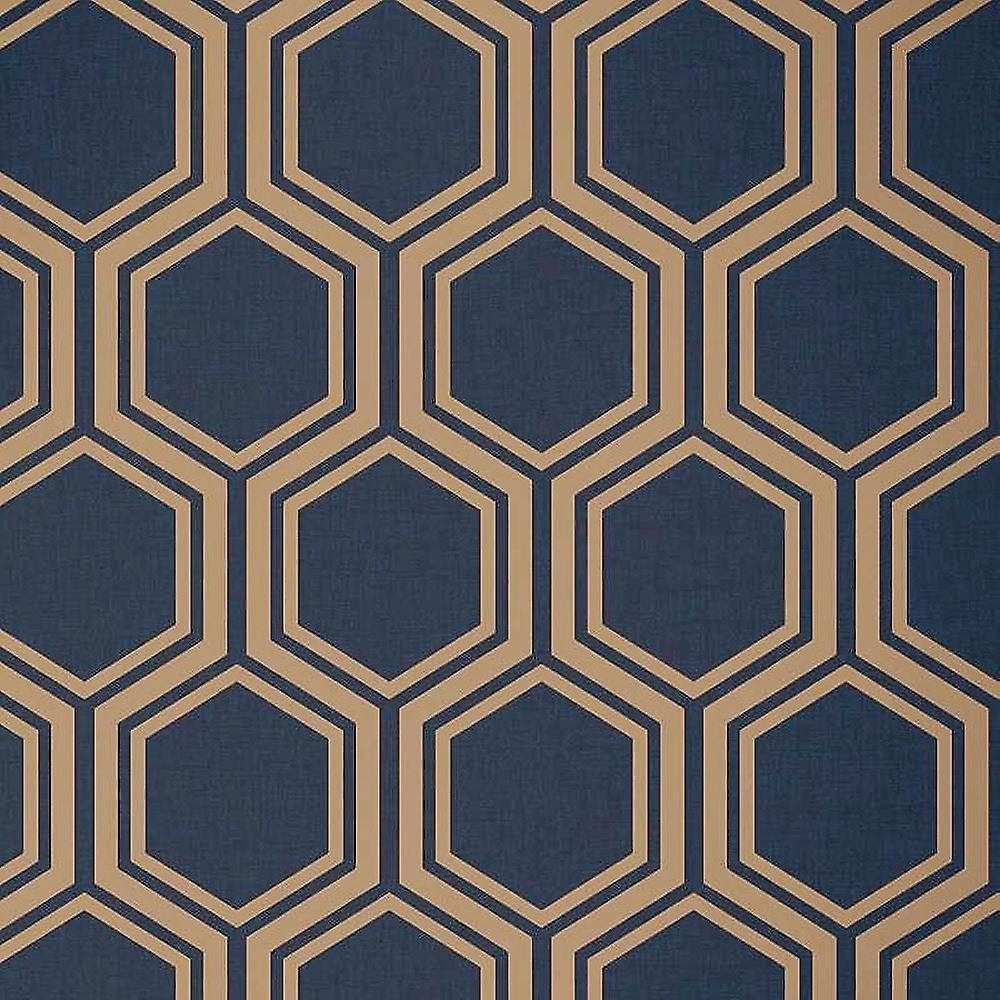
\includegraphics{images/geometric_design.jpg}} 
\vspace{.5cm}
\caption{Image reference for the geometric design of level 1.}
\label{fig:geometric}
\end{center}
\end{figure} 

In order to increase variation for users who cycle through the installation many times, easter eggs situated at several edge cases within each level.  For example, if a user places one hand on one side of the installation and the other hand at the other side a new color or feature may be displayed.  Users who spend more time will discover more easter eggs, but users who spend less time will still be able to interact with and enjoy the installation without feeling confused about how to operate the installation.  In order to aid with any confusion, there will be visual hints and motions to encourage user interaction. These hints will fade in after a certain amount of inactivity from the user, but will not interfere with user play if the user decides to explore one level instead of advancing. 

``Computational Queries'' seeks to explore the innate curiousity within each person as well as curated discoverability within any well-designed app and game. This exhibit aims to provide an avenue for exploration and accomplishment through play.The installation will allow users the flexibility to explore and discover new features and levels while also giving the users a sense of accomplishment when they discover something new even if it was not an advancement to the next level. As a whole, this installation intends to provide users with a carefree way to move their bodies, tap into their inner curiousity and problem solving skills, and enjoy a different mode of gameplay than they are used to. 


\section{Technical Background}
At the highest level, this installation focuses on human movement as the primary way of interacting with a computer.  This project will use handtrack.js, an open source hand tracking software developed by Victor Dibia \cite{noauthor_handtrackjs_nodate-1}, to interpret user movement as input for the computer.  This software will use the video feed from a webcam to create a bounding box around each instance of a human hand or face (Figure \ref{fig:bounding_boxes}).  

\begin{figure}[hbh]
\begin{center}
\scalebox{.4}{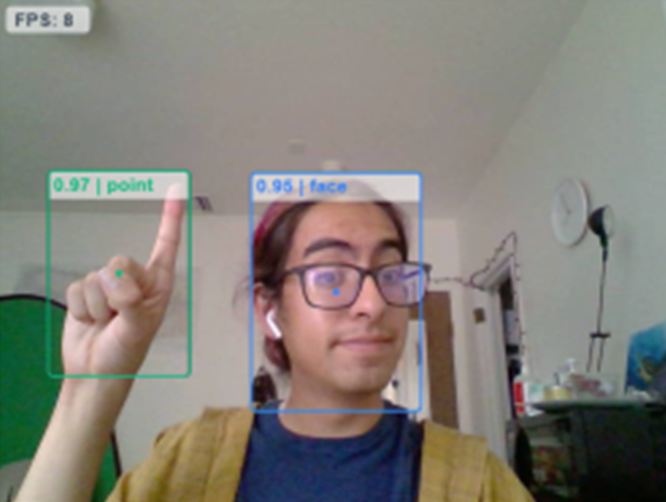
\includegraphics{images/bounding_example_resized.png}} 
\vspace{.5cm}
\caption{Classification and bounding boxes for a frame of a person}
\label{fig:bounding_boxes}
\end{center}
\end{figure}

It also classifies each hand as ``open'', ``closed'', ``pinch'', or ``point''.  Since handtrack.js is a JavaScript based package made for web applications, it makes sense to create this installation using HTML5, CSS3, and a webcam - elements that are common with most computers.   As a result, this installation may be repurposed as a web application for the general public after its run as an installation at Occidental College. 

Initial testing of handtrack.js revealed that it has a very small number of frames per second (FPS) that varies between 8FPS and 16FPS.  This fluctuation is based on how fast the recognition software can process each frame of the video input. More processing time = less frames outputted.  Fortunately, this is not a sequential delay in output (the cause of lag, also called first in, first out), but rather a first in, first out approach.  In this way, any frames that were missed as a result of the processing time are discarded and the next newest frame is processed.  Even though this approach does not interfere with continuity for the viewer, it produces a jerky video as a result of the reduction in FPS.  

The industry standard for high definition films is 24 FPS \cite{noauthor_3_nodate} which is the smallest number of FPS that creates smooth motion.  The proposed implementation of handtrack.js produces almost half of the industry standard which causes a jerky live video feed.  Fortunately, the individual bounding boxes create convincing continuous motion when the live video feed is removed and only the bounding boxes remain. In the final installation, these bounding boxes will also be removed and the movement of the pattern will cue the user in to where their hand is positioned in relation to the installation.  

Unfortunately, user motion needs to be fairly slow in order for the program to accurately identify the user's hands.  Since faster motion causes motion blur in photos, each individual frame will be blurred if the user moves quickly. As a result, the image recognition software is unable to correctly identify the bounding boxes of the hands since their shape is blurred. Further research suggests that an easy solution is to reduce the exposure time for each individual frame which will remove the blur \cite{e_adjusting_2019} and allow for better hand recognition.   

This project will also make use of the MVC architecture often used in games.  MVC stands for Model, View, Controller and details the way these three components interface with each other. In the MVC architecture, the user interfaces with the controller which sends information to the model.  The model then changes according to the controller and updates the view which the user observes.  Based on this update, the user will decide what action to take through the controller to continue the cycle. 

The model will be written in JavaScript and will interface with handtrack.js (the controller) and the view (the HTML output).  The view will be generated using the built in JavaScript canvas properties to create geometric patterns that shift and change according to user movements. 

\section{Prior Work}

\citetitle{kwon_real-time_nodate} by \citeauthor{kwon_real-time_nodate} highlights many interactive generative art exhibits from the early 2000s. In 2002, Scott Snibbe created a visualization that recorded users' shadows and played them back allowing the user to add new shadows to the playback loop - similar to a guitar feedback loop. 

\begin{figure}[hbh]
\begin{center}
\scalebox{.12}{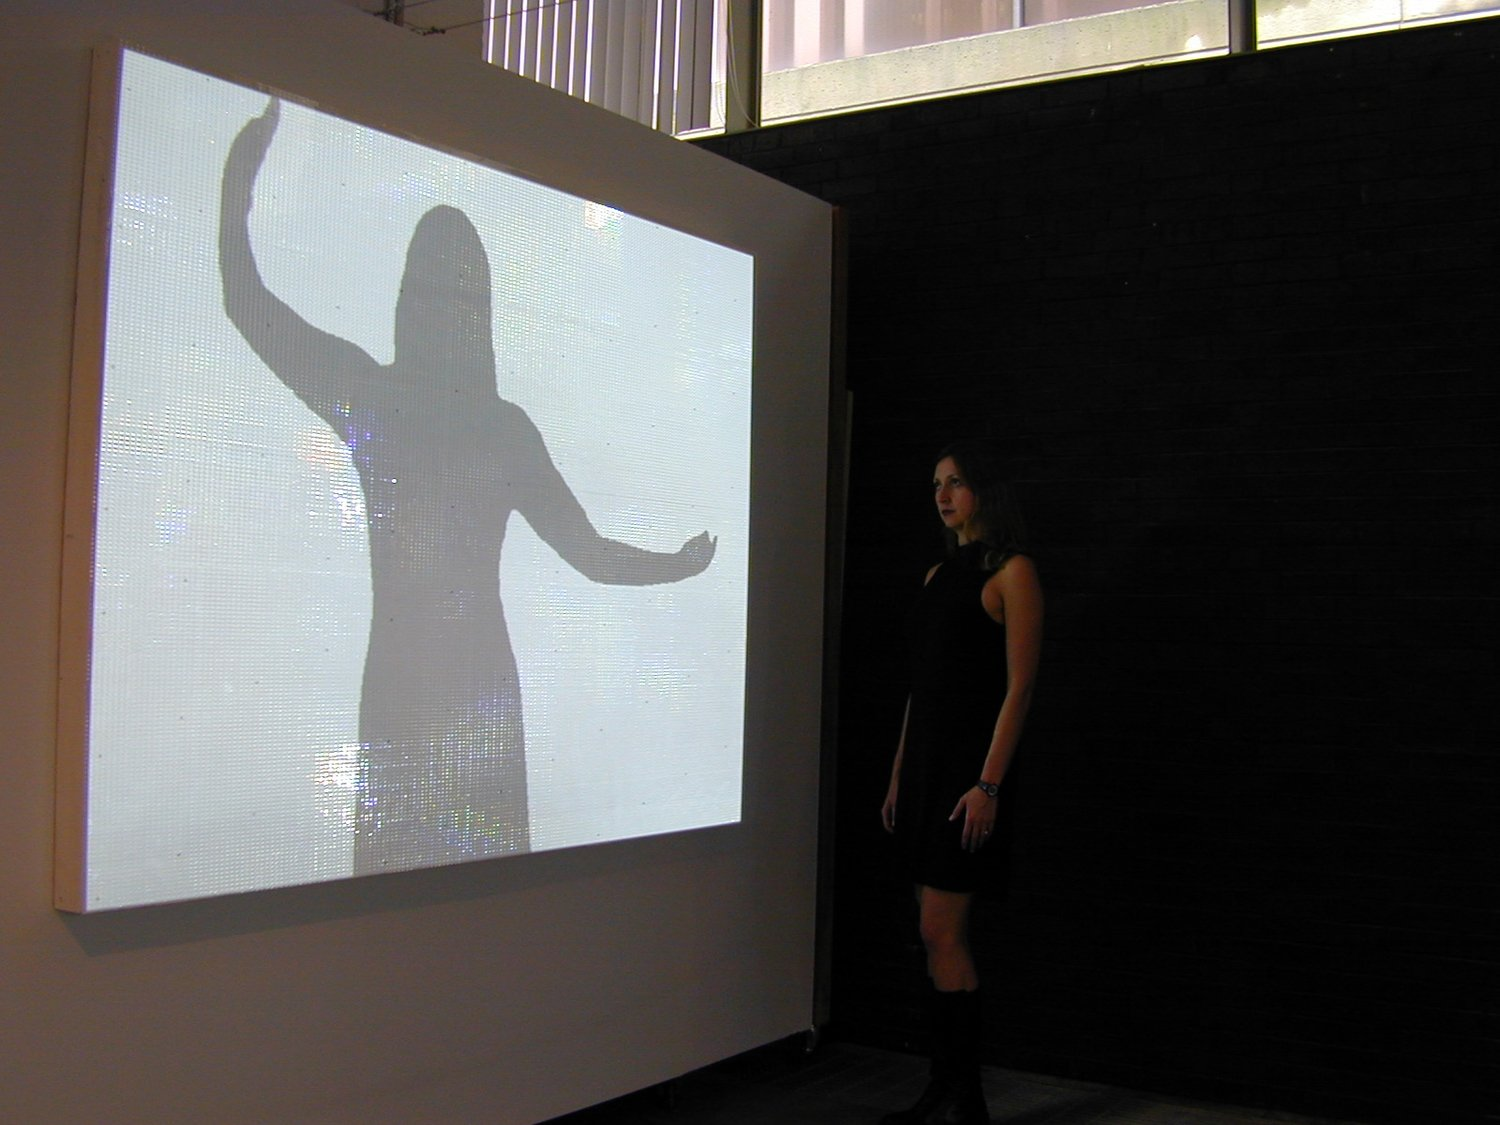
\includegraphics{images/shadow-2002.jpeg}} 
\vspace{.5cm}
\caption{A person watching Scott Snibbe's ``Shadow''. }
\label{fig:shadow-2002}
\end{center}
\end{figure} 

Then, in 2015, Philip Worthington created the installation ``Shadow Monsters`` which used machine learning to recognize specific shapes and features in a user's shadow and modify it too create a `monster' \cite{houston_public_media_mfah_2015}.  For example, shadows that look like circles will be made into the monster's eyes, and shadows that look like intersecting lines will be made into the monster's mouth.  This transformation happens in real time and artificial extremeties are added in real time to the user's shadow.

``Future You`` (2019) by Universal Everything, a technological art company, focuses on real time mirroring of the user to animate a unique CGI character \cite{noauthor_future_2019}. This CGI character is a humanoid, futuristic being that is unique for each user based upon predetermined variables. Additionally, this character undergoes an evolution every 5 seconds becoming more complex the longer a user interacts with it.  In this way, the program is generating and modifying the art based upon the user's actions according to various variables (time and appearance).  

``Computational Queries'' draws a lot of inspiration from Aakash Nihilani, an artist known for his 3D geometric illusions. Specifically, his interactive geometric series titled ``Projections'' from 2015 \cite{noauthor_aakash_nodate}.  These interactive projections incorporate different geometric patterns that flow and ebb as users run their hands along the wall that the projections are screened on. As these geometric patterns move, bright colors are revealed in the space between each shape.  This paper describes an art installation that uses various aspects from all of this previous work. 

\begin{figure}[hbh]
\begin{center}
\scalebox{.45}{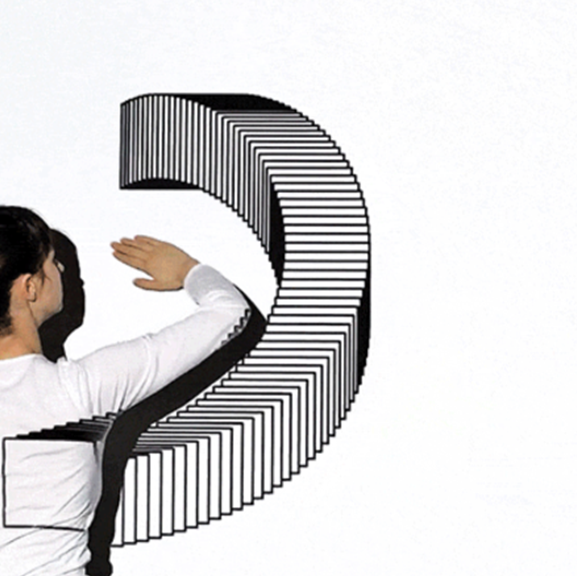
\includegraphics{images/squares-2015.png}} 
\vspace{.5cm}
\caption{A person interacting with Aakash Nihilani's ``Squares''. }
\label{fig:shadow-2002}
\end{center}
\end{figure} 

\section{Methods}
 A tutorial by Larry Sass-Ainsworth on medium.com \cite{sass-ainsworth_getting_2019} provides a good starting point to get handtrack.js up and running.  This tutorial covers how to add handtrack.js to any HTML project and provids source code for a functional, intuitive video feed that tracks face and hand positions. After following this tutorial, the JavaScript and HTML will be edited to remove the live video feed and to create the responsive pattern.  This pattern will move and respond to the position of the user's hand in the room as tracked by handtrack.js. 
 
Five different patterns will be generated algorithmically using the JavaScript canvas feature. Then, these patterns will be tweaked and edited to become interactive levels of the installation.  Additional frameworks will be added to allow users to acheive the next level through specific interactions.  These interactions could be a specific motion by the user, a movement at a particular portion of the screen, or a sequence of recognizable motions.  Then, various easter eggs based on extreme motions will be created with the intention of being discovered organically by the user. 

After a crude rendering of any one part of the above backend logic is completed, user testing will begin. User testing will commence after each new feature is completed and after any large portion of the installation has been changed. Following user testing, the installation will be revaluated according to the decided metrics and updated. Then, the cycle of testing and updating will repeat. 

After the backend logic has begun user testing, work on the frontend graphics will begin and be added to the cycle of user testing. 

\section{Evaluation Metrics}
\citetitle{bernhaupt_video_2010} by \citeauthor{bernhaupt_video_2010} suggests that user testing should be done at every stage of development and provides a framework for different types of testing: free flow, narrow specific, and broad specific. Free flow allows users to explore the exhibit at will and play as long as they are interested.  This provides a useful time based metric that will quantifiably express how interested users are.  Furthermore, this approach will highlight any portions of interaction that are unclear or confusing to users as they experience it in real time. This type of user testing will likely start once a crude version of the entire installation has been developed. 

Narrow specific asks users to focus on a specific part or action in the game and they play it over and over again which will help developers see different possible ways users will approach the same task as well as any potential bugs from repeated play. This type of testing will commence after any new feature is developed and integrated into the installation. 

Broad specific is similar to narrow specific, but focuses on a larger portion of the exhibit.  It asks players to complete a longer task, but still requires them to complete it repetitively. This type of testing will be useful as more connected parts of the installation are created. For example, once both level one and level two are done, broad specific can be used to see how the player reacts after playing the first level and succeeding to the second level. 

As a whole, these three metrics will provide valuable qualitative and quantitative data regarding different portions of the game. Furthermore, this comprehensive test will highlight any confusing portions of the game and expose any bugs through repeated gameplay. 

\section{Ethical Considerations}

\subsection{Ethical Design}\label{sec:design}

In the textbook ``Introduction to Art: Design, Context, and Meaning,'' \cite{blood_introduction_nodate}the authors caution against different types of unethical practices when creating an art piece. \citeauthor{blood_introduction_nodate} warns against `appropriation' or the act of incorporating another artist's work into their own without any change or edits and without acknowledgement or credit. Similar to plagarism, this type of artistic appropriation not only steals intellectual property from the original artist, but also damages the credibility of the emerging artist.  While artists often borrow ideas, aesthetics, or even entire pieces from other artists, ``Introduction to Art...'' makes the distinction that these artists are intentionally altering the original idea in order to comment on it's original meaning or to recontextualize it in a new setting. In this way, new artists are still bringing their own intentions and ideas to the original work.  

As mentioned above, this project draws a lot of inspiration from Aakash Nihilani.  While Nihilani's projection work focuses on interactive geometric works,``Computational Queries'' will ask users to wave their hands in front of geometric patterns in order to reveal another `level' of the game.  Even though ``Computational Queries'' will have a different color scheme and type of user interaction than ``Projections,'' the two installations are still very similar in structure and topic.  As such, the final installation will offer a special thanks or acknowledgement for Aakash Nihilani as an inspiration for this work. 

\subsection{Ethical Interaction}\label{sec:interaction}

As mentioned, this installation focuses on human movement as input.  Unfortunately, not all users will be able to interact with the installation.  Hand amputees will not be able to advance to the next level or cause changes to the installation since the hand tracking software will not be able to accurately capture their arm movements. Furthermore, users with motor inhibitions may not be able to accurately complete the motions needed to advance to the next level.  These motions could include moving hands from side to side, or bringing hands together and apart again; motions that are not possible for every user. 

Providing additional ways to interact with the piece becomes integral when dealing with differently abled people. For example, a joystick controller, handheld mouse, or eye tracking software as inputs to determine the position of the movement allows differently abled people alternative ways to interact that don't involve their hands. This type of interaction is necessary to advance through the installation, however, differently abled people will still be able to experience the installation by watching someone else interact in real time. Unfortunately, this is not possible for blind/low vision people. 

This installation relies heavily on visual feedback for the user.  Users are visually instructed how to interact with the exhibit and then, when they are interacting, the installation responds to their movements by visually updating the displayed projection.  Furthermore, people who interact with the exhibit will be visually prompted with hints on screen as well as given visual feedback as a metric for success through the levels. As such, users with visual impairments will not experience any sensory differences as they physically interact with the installation.  For all intents and purposes, they will have walked into an empty room and nothing will signal that anything has changed. 

In order to account for this, a compelling soundscape that changes as a user interacts can mimic the visual outputs aurally. For example, as the user interacts with the pattern by moving their hands, the music could change or add a sound.  In this way, blind and low vision users can still interact with the exhibit. Furthermore, these sounds could also move to different speakers throughout the room, a technique that could motivate blind/low vision people to move around the space which would further change the audio landscape. 

\section{Timeline}
After a brief break in May, this summer will be spent doing more in depth research about the geometric patterns that can be created algorithmically using JavaScript.  This research will also include the design and artist's renditions of the different levels.  In addition, the specific easter eggs and mechanics of advancing to the next level (gameplay) will be designed. Lastly, more research into discoverability from a UI/UX lens will be done so that specific user hints and nudges can be designed and artistically rendered.  

Starting August 1st, the above progress will be finalized and backend development will begin regarding the generation of crude responsive visuals based upon an input of user movement.  The advancement from one level to another may also be tested during this time. 

On August 15th, work to create a crude version of the entire installation should begin and a crude playable version should be developed by the end of August. 

The first half of September will be dedicated to front end development of realizing the proposed designs from the summer. During this time, initial user testing will occur on the crude playable game. 

A final first version of both the backend and frontend of the project will be realized by the end of September. 

In depth user testing will begin on October 1st and the game will be updated and improved throughout October.  Initial design and content for the poster will also be completed by October 31st and updated as data is analyzed from user testing. 

User testing and the final poster will be completed before Thanksgiving break and final edits, debugging, and tweaks will be finalized by December 1st. After Thanksgiving break, documentation for the code will be written on the github page for the project. 

December 1st-5th will consist of preparation for the poster presentation.  December 6th-15th will be dedicated to writing and revising the final senior comprehensive paper. 

\printbibliography 

\end{document}
